\documentclass[11pt,a4paper]{report}
\usepackage[margin=1in]{geometry}
\usepackage[T1]{fontenc}
\usepackage{lmodern}
\usepackage{hyperref}
\usepackage{booktabs}
\usepackage{longtable}
\usepackage{listings}
\usepackage{xcolor}
\usepackage{graphicx}
\usepackage{tikz}
\usetikzlibrary{shapes,arrows.meta,positioning}

\hypersetup{colorlinks=true,linkcolor=blue,urlcolor=blue}
\lstdefinestyle{bash}{
  basicstyle=\ttfamily\small,
  breaklines=true,
  frame=single,
  backgroundcolor=\color{gray!8}
}

\title{CXR Redis Lab Manual\\
\large SW.14 --- Redis + Redis Insight + cache-aside\\
\large Full implementation record}
\author{CXR Ops Lab --- \texttt{cxr-ops-lab}}
\date{2026-05-31}

\begin{document}
\maketitle
\begin{abstract}
Complete bootcamp record for \textbf{SW.14}: every file added for \textbf{Redis (:6379)},
\textbf{Redis Insight (:5540)}, the \textbf{cache-aside} shell demo, how keys connect to
\textbf{Claim Studio (:3000)} conceptually, and troubleshooting from the live lab session
(empty browser, \texttt{127.0.0.1} vs \texttt{redis}, TTL expiry, second-run \texttt{DEL}).
\end{abstract}
\tableofcontents
\newpage

\chapter{What Redis does in CXR (vs other observe labs)}

\begin{center}
\begin{tabular}{llll}
\toprule
Pattern & Tool & URL & SW \\
\midrule
Metrics & Grafana & :3001 & SW.10 \\
Traces & Jaeger & :16686 & SW.11 \\
Logs & Kibana & :5601 & SW.12 \\
Async events & Kafka / Kafka UI & :9092 / :8082 & SW.13 \\
\textbf{Hot read cache} & \textbf{Redis + Insight} & \textbf{:6379 / :5540} & \textbf{SW.14} \\
\bottomrule
\end{tabular}
\end{center}

\noindent\textbf{Claim Studio} (\url{http://localhost:3000/claim-studio}) is the product dashboard.
\textbf{Redis is not embedded} in the Next.js app in this lab --- a standalone script demonstrates
\textbf{cache-aside} against a static JSON artifact that matches the Kafka event schema.

\chapter{Architecture: cache-aside end-to-end}

\section{Data flow}

\begin{center}
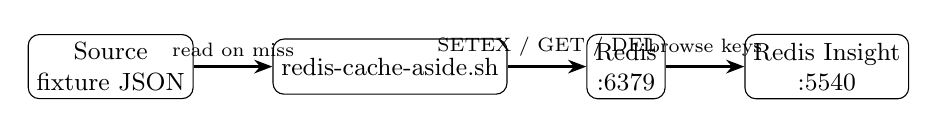
\begin{tikzpicture}[
  node distance=0.6cm and 0.45cm,
  box/.style={draw, rounded corners, minimum height=0.7cm, align=center, font=\small, inner sep=3pt},
  arr/.style={-{Stealth}, thick}
]
  \node[box] (src) {Source\\fixture JSON};
  \node[box, right=1cm of src] (script) {redis-cache-aside.sh};
  \node[box, right=1cm of script] (redis) {Redis\\:6379};
  \node[box, right=1cm of redis] (insight) {Redis Insight\\:5540};
  \draw[arr] (src) -- node[above,font=\scriptsize]{read on miss} (script);
  \draw[arr] (script) -- node[above,font=\scriptsize]{SETEX / GET / DEL} (redis);
  \draw[arr] (redis) -- node[above,font=\scriptsize]{browse keys} (insight);
\end{tikzpicture}
\end{center}

\section{Cache-aside steps (syllabus)}

\begin{enumerate}
  \item \texttt{GET cxr:claim:analyzed:\{claim\_id\}} --- miss returns \texttt{(nil)}.
  \item Load \texttt{lab/fixtures/claim-analyzed.demo.json} (stand-in for DB/API after analyze).
  \item \texttt{SETEX key TTL json} --- default TTL \textbf{300s}.
  \item \texttt{GET} --- cache hit on repeat read.
  \item \textbf{Invalidation:} \texttt{DEL key} on update (second script run when key is warm).
\end{enumerate}

Mermaid source: \texttt{docs/diagrams/06-redis-cache-aside.mmd}.

\section{Cached key and payload}

\begin{center}
\begin{tabular}{ll}
\toprule
Item & Value \\
\midrule
Key & \texttt{cxr:claim:analyzed:demo-1} \\
Type & STRING \\
Fixture & \texttt{lab/fixtures/claim-analyzed.demo.json} \\
Schema & \texttt{schemas/cxr.claim-analyzed.v1.json} \\
TTL env & \texttt{CXR\_CACHE\_TTL\_SEC} (default 300) \\
\bottomrule
\end{tabular}
\end{center}

\chapter{Docker stack (\texttt{compose.redis.yaml})}

\section{Services}

\begin{longtable}{@{}p{3.2cm}p{4cm}p{7cm}@{}}
\toprule
Service & Image & Role \\
\midrule
\endhead
\texttt{redis} & \texttt{redis:7.4-alpine} & Cache server; published \textbf{:6379}; no persistence (\texttt{--save ""}, no AOF) \\
\texttt{redis-insight} & \texttt{redis/redisinsight:2.70} & Web UI \textbf{:5540}; volume \texttt{redis\_insight\_data} \\
\bottomrule
\end{longtable}

\section{Why two ports?}

\begin{center}
\begin{tabular}{lll}
\toprule
Port & Protocol & Browser? \\
\midrule
6379 & Redis (RESP) & \textbf{No} --- use \texttt{redis-cli} or Insight \\
5540 & HTTP (Insight UI) & \textbf{Yes} --- Simple Browser / Chrome \\
\bottomrule
\end{tabular}
\end{center}

\chapter{Redis Insight --- connect and browse (highlight)}

\section{Start stack}
\begin{lstlisting}[style=bash]
cd cxr-ops-lab
./scripts/17-redis-up.sh
./lab/redis-cache-aside.sh
\end{lstlisting}

\section{Open UI in Cursor}
\begin{enumerate}
  \item \textbf{Ctrl+Shift+P} $\rightarrow$ \textbf{Simple Browser: Show}
  \item URL: \url{http://localhost:5540}
  \item Allow $\sim$30s on first boot if smoke warns ``Insight not ready''.
\end{enumerate}

\section{Add database (first time only)}

\textbf{Wrong (common):} Connection URL \texttt{redis://default@127.0.0.1:6379}\\
Insight runs \emph{inside} Docker; \texttt{127.0.0.1} is Insight's own container, not Redis.

\textbf{Correct:}
\begin{lstlisting}[style=bash]
redis://redis:6379
\end{lstlisting}
Or \textbf{Connection Settings}: Host \texttt{redis}, Port \texttt{6379}, alias \texttt{cxr-lab}.

Linux fallback if needed: \texttt{redis://host.docker.internal:6379} (Redis published on host :6379).

\section{Golden path in UI}

\begin{enumerate}
  \item Run \texttt{./lab/redis-cache-aside.sh} \textbf{once} (creates key).
  \item Insight $\rightarrow$ database \texttt{redis:6379} $\rightarrow$ \textbf{db0} $\rightarrow$ refresh.
  \item Click \texttt{cxr:claim:analyzed:demo-1} --- JSON + TTL on right pane.
  \item Screenshot: \texttt{evidence/SW14-redis-insight-2026-05-31.png}
\end{enumerate}

\textbf{Do not} use ``Load sample data'' --- unrelated demo keys.

\section{Longer TTL for screenshots}
\begin{lstlisting}[style=bash]
CXR_CACHE_TTL_SEC=3600 ./lab/redis-cache-aside.sh
\end{lstlisting}

\chapter{Step-by-step procedure (CLI + UI)}

\section{Step 1 --- Start Redis + Insight}
\begin{lstlisting}[style=bash]
./scripts/17-redis-up.sh
\end{lstlisting}

\section{Step 2 --- Cache-aside demo}
\begin{lstlisting}[style=bash]
./lab/redis-cache-aside.sh          # miss -> load -> SETEX -> hit
./lab/redis-cache-aside.sh          # warm key -> DEL (invalidation)
\end{lstlisting}

\section{Step 3 --- Smoke test}
\begin{lstlisting}[style=bash]
./scripts/17-redis-smoke.sh
\end{lstlisting}
Expect: \texttt{PONG}, Insight :5540 (or WARN wait 30s), \texttt{CACHE HIT}.

\section{Step 4 --- Manual redis-cli (optional)}
\begin{lstlisting}[style=bash]
docker exec -it cxr-ops-lab-redis-1 redis-cli ping
docker exec -it cxr-ops-lab-redis-1 redis-cli GET cxr:claim:analyzed:demo-1
docker exec -it cxr-ops-lab-redis-1 redis-cli TTL cxr:claim:analyzed:demo-1
\end{lstlisting}

\section{Step 5 --- Evidence}
\begin{itemize}
  \item \texttt{evidence/SW14-redis-verify-2026-05-31.md} --- all checkboxes
  \item \texttt{evidence/SW14-redis-insight-2026-05-31.png} --- Insight with JSON visible
\end{itemize}

\section{Step 6 --- Stop (optional)}
\begin{lstlisting}[style=bash]
docker compose -f compose.redis.yaml down
\end{lstlisting}

\chapter{Files created and touched (full inventory)}

\section{New files (SW.14)}

\begin{longtable}{@{}p{5cm}p{8cm}@{}}
\toprule
File & Purpose \\
\midrule
\endhead
\texttt{compose.redis.yaml} & Redis + Redis Insight compose \\
\texttt{lab/redis-cache-aside.sh} & Cache-aside demo (GET/SETEX/DEL) \\
\texttt{lab/fixtures/claim-analyzed.demo.json} & CXR-shaped cache payload \\
\texttt{scripts/17-redis-up.sh} & \texttt{compose.redis.yaml up -d}; prints :6379 and :5540 \\
\texttt{scripts/17-redis-smoke.sh} & PING, Insight probe, cache-aside check \\
\texttt{scripts/build-redis-manual-pdf.sh} & Builds this PDF \\
\texttt{docs/CXR-REDIS-LAB-MANUAL.md} & Markdown twin \\
\texttt{docs/CXR-REDIS-LAB-MANUAL.tex} & LaTeX source \\
\texttt{docs/CXR-REDIS-LAB-MANUAL.pdf} & Printable record \\
\texttt{docs/diagrams/06-redis-cache-aside.mmd} & Sequence diagram \\
\texttt{evidence/SW14-redis-verify-2026-05-31.md} & Verify checklist \\
\texttt{evidence/SW14-redis-insight-2026-05-31.png} & User UI screenshot \\
\bottomrule
\end{longtable}

\section{Related (not modified for Redis wiring)}

\begin{longtable}{@{}p{5cm}p{8cm}@{}}
\toprule
File & Note \\
\midrule
\endhead
\texttt{schemas/cxr.claim-analyzed.v1.json} & Same event shape as SW.13 Kafka sample \\
\texttt{compose.yaml} / \texttt{cxr-ui} & Claim Studio :3000 --- not calling Redis yet \\
\texttt{docs/PLATFORM-SYLLABUS-MAP.md} & SW.14 row updated \\
\bottomrule
\end{longtable}

\chapter{Environment variables}

\begin{center}
\begin{tabular}{lll}
\toprule
Variable & Default & Effect \\
\midrule
\texttt{CXR\_CACHE\_CLAIM\_ID} & \texttt{demo-1} & Key suffix \\
\texttt{CXR\_CACHE\_TTL\_SEC} & \texttt{300} & SETEX seconds \\
\texttt{CXR\_CACHE\_ARTIFACT} & fixture path & JSON source file \\
\bottomrule
\end{tabular}
\end{center}

\chapter{Troubleshooting (from live session)}

\begin{itemize}
  \item \textbf{Browser on :6379 fails} --- expected; Redis is not HTTP. Use :5540 or \texttt{redis-cli}.
  \item \textbf{Insight connect fails with 127.0.0.1} --- use host \texttt{redis} or URL \texttt{redis://redis:6379}.
  \item \textbf{Key in list but ``does not exist''} --- TTL expired or second script run DEL'd key; re-run cache-aside once; refresh UI.
  \item \textbf{Empty db0 / 0 keys} --- same; run \texttt{./lab/redis-cache-aside.sh}; refresh; avoid running script twice in a row before screenshot.
  \item \textbf{Smoke WARN Insight not ready} --- wait 30s; reload \url{http://localhost:5540}.
  \item \textbf{Container filter} --- scripts target \texttt{cxr-ops-lab-redis-1} (not \texttt{redis-insight}).
\end{itemize}

\chapter{ADR: where Redis fits CXR production}

\textbf{Good cache candidates:} reference codes, static policy snippets, \emph{completed} analyze snapshots with TTL.\\
\textbf{Risky:} caching in-flight \textbf{Run Analysis} without invalidation --- stale approvals/denials.\\
\textbf{This lab:} script-only; no Next.js \texttt{ioredis} on :8251 or :3000.

\chapter{Port map (CXR lab)}

\begin{center}
\begin{tabular}{lll}
\toprule
Port & Service & SW.14 \\
\midrule
3000 & Claim Studio & Source of truth (not cached yet) \\
6379 & Redis & Cache API \\
5540 & Redis Insight & \textbf{Web UI} \\
8251 & Rehearsal dev & Unchanged \\
8082 & Kafka UI & SW.13 \\
5601 & Kibana & SW.12 \\
16686 & Jaeger & SW.11 \\
\bottomrule
\end{tabular}
\end{center}

\chapter{Study plan linkage}

\begin{center}
\begin{tabular}{ll}
\toprule
Item & Maps to \\
\midrule
SW.14 syllabus row & Cache-aside + TTL + invalidation \\
User verify & \texttt{SW14-redis-verify-2026-05-31.md} \\
After SW.14 & SW.15+ electives \\
\bottomrule
\end{tabular}
\end{center}

\chapter{Live adjustments (Redis Insight baked in)}

\begin{itemize}
  \item Added \texttt{redis-insight} service to \texttt{compose.redis.yaml} --- UI on \textbf{:5540} (Redis :6379 has no browser UI).
  \item Insight connect URL \texttt{redis://redis:6379} --- \textbf{not} \texttt{127.0.0.1} (Insight runs inside Docker network).
  \item Scripts filter container \texttt{cxr-ops-lab-redis-1} --- avoids matching \texttt{redis-insight} container.
  \item Second \texttt{redis-cache-aside.sh} run \textbf{DEL}s warm key --- re-run once before UI screenshot.
  \item \texttt{CXR\_CACHE\_TTL\_SEC=3600} optional for long screenshot windows.
\end{itemize}

\chapter{UI evidence --- Redis Insight (:5540)}

Key \texttt{cxr:claim:analyzed:demo-1} with CXR JSON payload and TTL.

\begin{figure}[htbp]
\centering
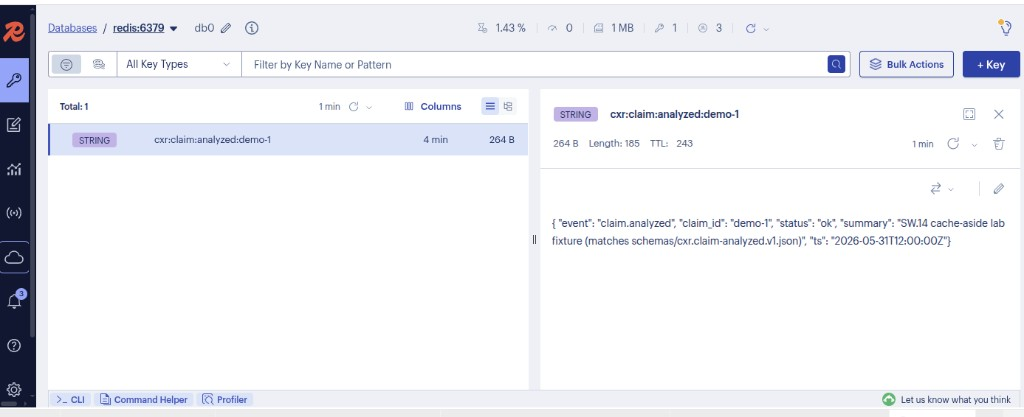
\includegraphics[width=0.92\textwidth]{../evidence/SW14-redis-insight-2026-05-31.png}
\caption{Redis Insight --- cached claim-analyzed JSON (SW.14 evidence).}
\end{figure}

\end{document}
